\section{Introduction}

The South Slavic languages, spoken mostly in the Balkans, make up one of the three Slavic 
branches. The South Slavic branch is in turn comprised of two subgroups, the Eastern 
subgroup containing Macedonian and Bulgarian, and the western subgroup containing 
Serbo-Croatian and Slovene.

The Serbo-Croatian dialects are the native language of most people in Serbia, Croatia, 
Montenegro and Bosnia and Herzegovina. They were formed on the basis of the Štokavian dialects 
which got their name from the form "što" (or "šta"), which is used for the interrogative pronoun "what?". A second group of dialects from the Serbo-Croatian language group is the Čakavian group spoken in western Croatia, Istria, the coast of Dalmatia, and some islands in the Adriatic. Like the Štokavian dialects, the Čakavian dialects got their name from the form "ča" used for the interrogative pronoun "what?". Finally, the third main group of Serbo-Croatian dialects, spoken in northwestern Croatia, uses kaj instead of "što", and is therefore called Kajkavian.
An intermediate between the Serbo-Croatian, Bulgarian and Macedonian is the Torlakian dialect.

The three or four standardised varieties of Serbo-Croatian are all based on the Štokavian dialect.

Slovenian is the native language of Slovenia, and is also spoken in the neighbouring areas in Italy and Austria. While Slovenian has many different dialects, it shares some features with the Kajkavian dialects spoken in Croatia. Although the speakers of the different Serbo-Croatian dialects can understand each other without any serious difficulties, a Serbo-Croatian speaker can have a difficult time understanding a speaker of a Slovene dialect.

\begin{figure}

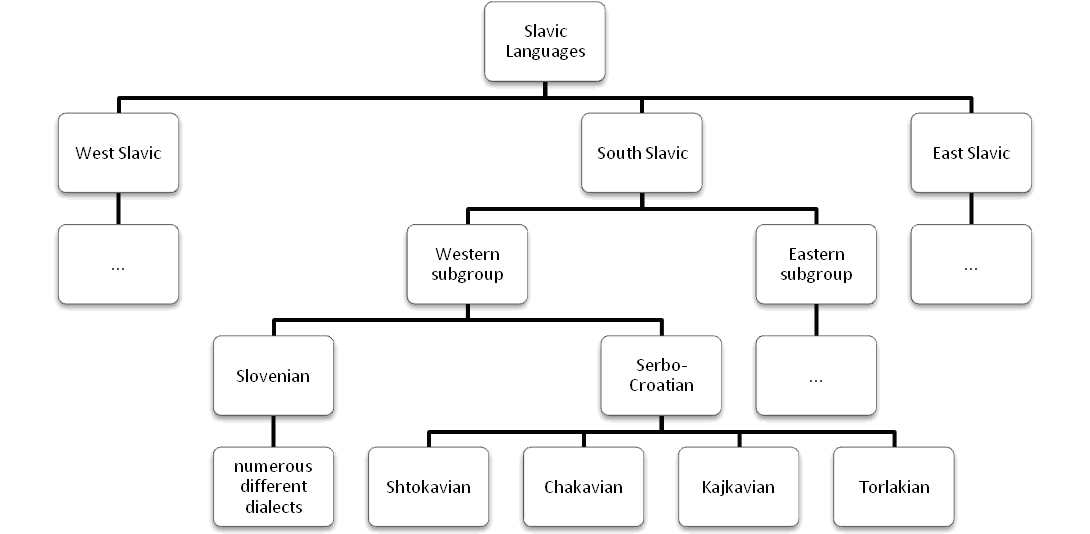
\includegraphics[scale=0.3]{images/chart.png}

\end{figure}


\begin{figure}

\todo{Venn diagram of Serbo-Croatian, Serbian, Croatian, Bosnian, Montenegrin, 
Neo-Štokavian, Čakavian, Kajkavian, Torlakian
Ekavian, Ijekavian, Ikavian}

\end{figure}

